\chapter{Что такое OTP?}
\label{what-is-otp}
\section{Это Открытая Телекоммуникационная Платформа!}
\label{its-the-open-telecom-platform}

\begin{wrapfigure}{l}{0.35\linewidth}
    
\includegraphics[width=1\linewidth]{hullo.png}
\end{wrapfigure}
OTP можно расшифровать как \emph{Открытая Телекоммуникационная Платформа}, хотя с телекоммуникациями она уже не так сильно связана, как прежде (она больше связана с программами, которые решают задачи, характерные для сферы телекоммуникаций).
Если сказать, что половина величия Erlang проистекает из его параллелизма (concurrency) и распределённости, а вторая половина заключена в его средствах обработки ошибок, то третьей половиной будет OTP фреймворк.

В предыдущих главах мы рассмотрели несколько примеров общих правил, которые используют при создании параллельных (concurrent) приложений, применяя встроенные средства языка: связи (links), мониторы, серверы, таймауты, улавливающие завершения (trapping exits), и т.д.
То и дело мы натыкались на подводные камни, и придумывали пути их обхода.
Говорили о том, как избежать состояний гонки (race conditions), а также о том, как важно не забывать, что процесс может умереть в любой момент.
Среди всего прочего мы также столкнулись с горячей загрузкой кода, именованием процессов и добавлением супервизоров.

Если делать всё перечисленное вручную, приходится тратить много времени, и при этом очень легко допустить ошибку.
Есть немало граничных случаев, о которых можно забыть, и множество ловушек, в которые легко угодить.
Фреймворк OTP справляется с этим вопросом, группируя жизненно важные принципы в набор библиотек, которые подверглись тщательной проектировке и годами закалялись в боях.
Их должен использовать каждый программист на Erlang.

Фреймворк OTP также включает набор модулей и стандартов, призванных помогать разработчику при построении приложения.
Если допустить, что большинство программистов на Erlang в конце концов приходят к использованию OTP, то большинство приложений, с которыми вы сможете столкнуться, будут склонны к следованию этим стандартам. 
\section{Обычный процесс в обобщении}
\label{the-common-process-abstracted}
Одним из общих приёмов, который мы многократно применяли в предыдущих примерах с процессами, было разделение всего что только можно в соответствии с очень конкретными задачами.
В большинстве процессов имеется функция, отвечающая за порождение нового процесса, функция, которая заведовала выдачей процессу начальных значений, основного цикла и т.д.

Оказывается, эти части обычно присутствуют во всех параллельных (concurrent) программах, которые вы будете писать, не взирая на назначение процесса.
\begin{figure}[h!]
    \centering
    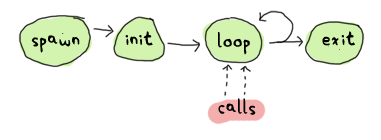
\includegraphics[width=0.7\textwidth]{common-pattern.png}
\end{figure}

Инженеры и учёные\--информатики, которые занимались разработкой OTP, выявили эти шаблоны и включили их в состав нескольких общих библиотек.
Эти библиотеки содержат код, эквивалентный большинству абстракций, использованных нами (таких как, к примеру, использование ссылок для пометки сообщений), с тем преимуществом, что этот код годами используется в работе и был построен с намного большей предусмотрительностью, чем наша реализация.
В их состав входят функции для безопасного порождения и инициализации процессов, отсылки сообщений с устойчивостью к сбоям и многое другое.
Забавно то, что вам редко придётся использовать эти библиотеки самостоятельно.
Те обобщения, которые они содержат, настолько просты и универсальны, что на их основе были построены намного более интересные вещи.
Вот такими библиотеками мы и воспользуемся.
\begin{figure}[h!]
    \centering
    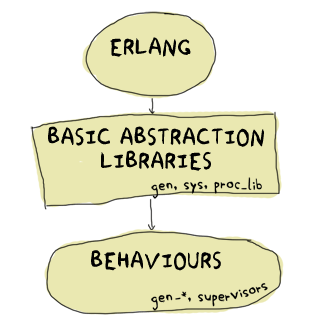
\includegraphics[width=0.65\textwidth]{abstraction-layers.png}
\end{figure}
В последующих главах мы столкнёмся с несколькими распространёнными приёмами использования процессов, а затем увидим как их можно обобщить и сделать универсальными.
Затем мы рассмотрим реализацию каждого из этих приёмов с помощью шаблонов поведения фреймворка OTP (OTP framework's behaviours), и увидим как их можно использовать.
